\chapter{Parsing}

After Lexical Analysis is complete and the input string has been tokenised the next step is to generate a parse tree.  Parsers produce a data structure that takes into account all the details of the language defied in its grammar and also attempt to perform error handing.

\section{Parse Trees}

A parser takes the output from lexical analysis and turns it into a data structure, as implied by the name this generally takes the form of a tree. 





\section{Parsing Blazon}

Parsing Blazon involves taking the tokens generated form Lexical analysis and producing a well formed data structure that checks whether the input conforms to the defied grammar or not and attempts to report the reason behind why the input may be erroneous.

Blazon lends it self very well to a top down, left to right parsing method because of the way the language is defined. Fields are defined and Tinctured from the top-left most point downwards and mirroring this approach in parsing makes for a nice parallel. 

The output from the lexical analysis is of a fairly high level because of the more advanced lexing approach taken which wrapped Line Types, Quantifiers and Tinctures into other objects when appropriate.  

To build the data structure itself each of the objects to be instantiated have inbuilt class variables to allows them to act as nodes in a tree. 

Partitions all have an array, the size of which is determined by the number of fields to be created for the particular type of partition.  Tinctures have an array of Charges so that they can have multiple charges placed upon them. 

As Blazon sentences all implicitly start with an empty field that encompass the entire shied this is where the parser and parse tree will start.  In the implementation the implicit field is represented by a partition which produces a single field,  an \emph{Escutcheon}. 

The parser then takes the first token, according to the grammar the only valid operations that can be performed upon a field are Tincturing it or Partitioning it, therefore the parser checks whether this token is either a Tincture or a Partition and if it either of the above adds it to the initial field accordingly.  

This process is repeated until either there are no more tokens left to parse or there is no more space in the tree structure or ideally both. 



\section{Parsing Example}

 
The following demonstrates the parsing of the Blazon sentence \emph{Per Bend Azure and Or a Cross Vert}.  

The tokens generated by Lexical analysis would be 


\begin{figure}[H]
  \centering
    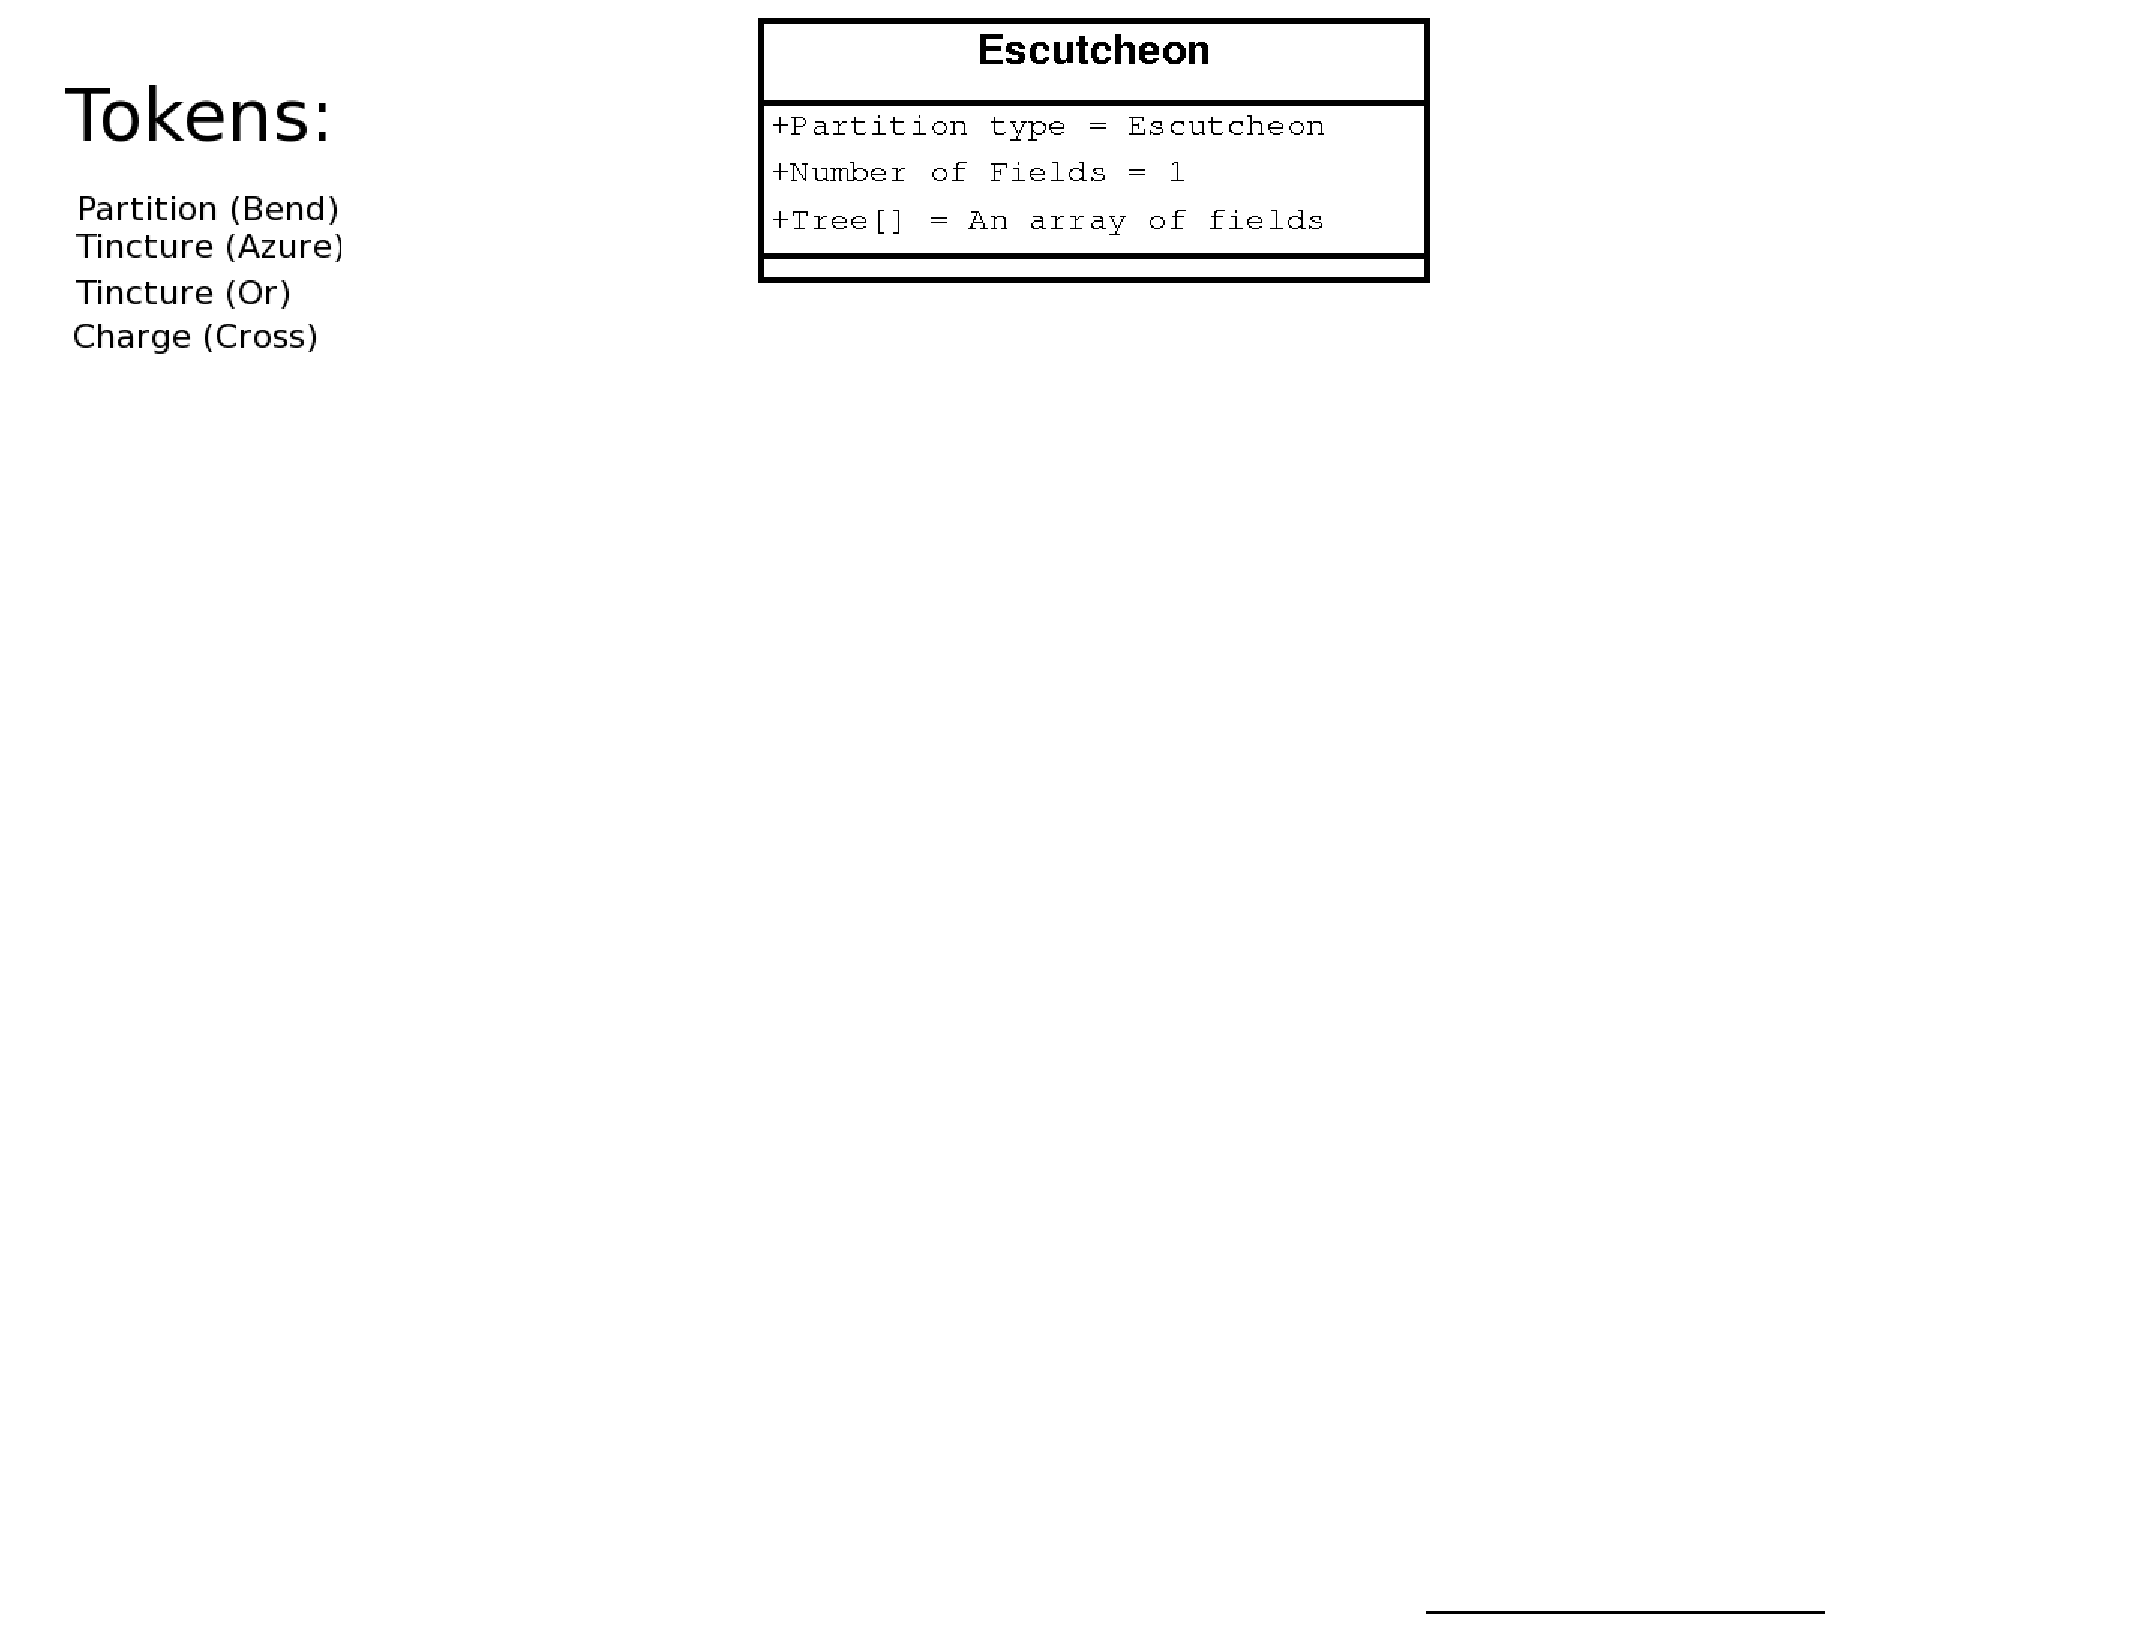
\includegraphics[width=0.8\textwidth]{parsing/images/Parsing5.eps}
  \caption{\emph{"The root of the tree is the implicit Field."}}
  
\end{figure}


\begin{figure}[H]
  \centering
    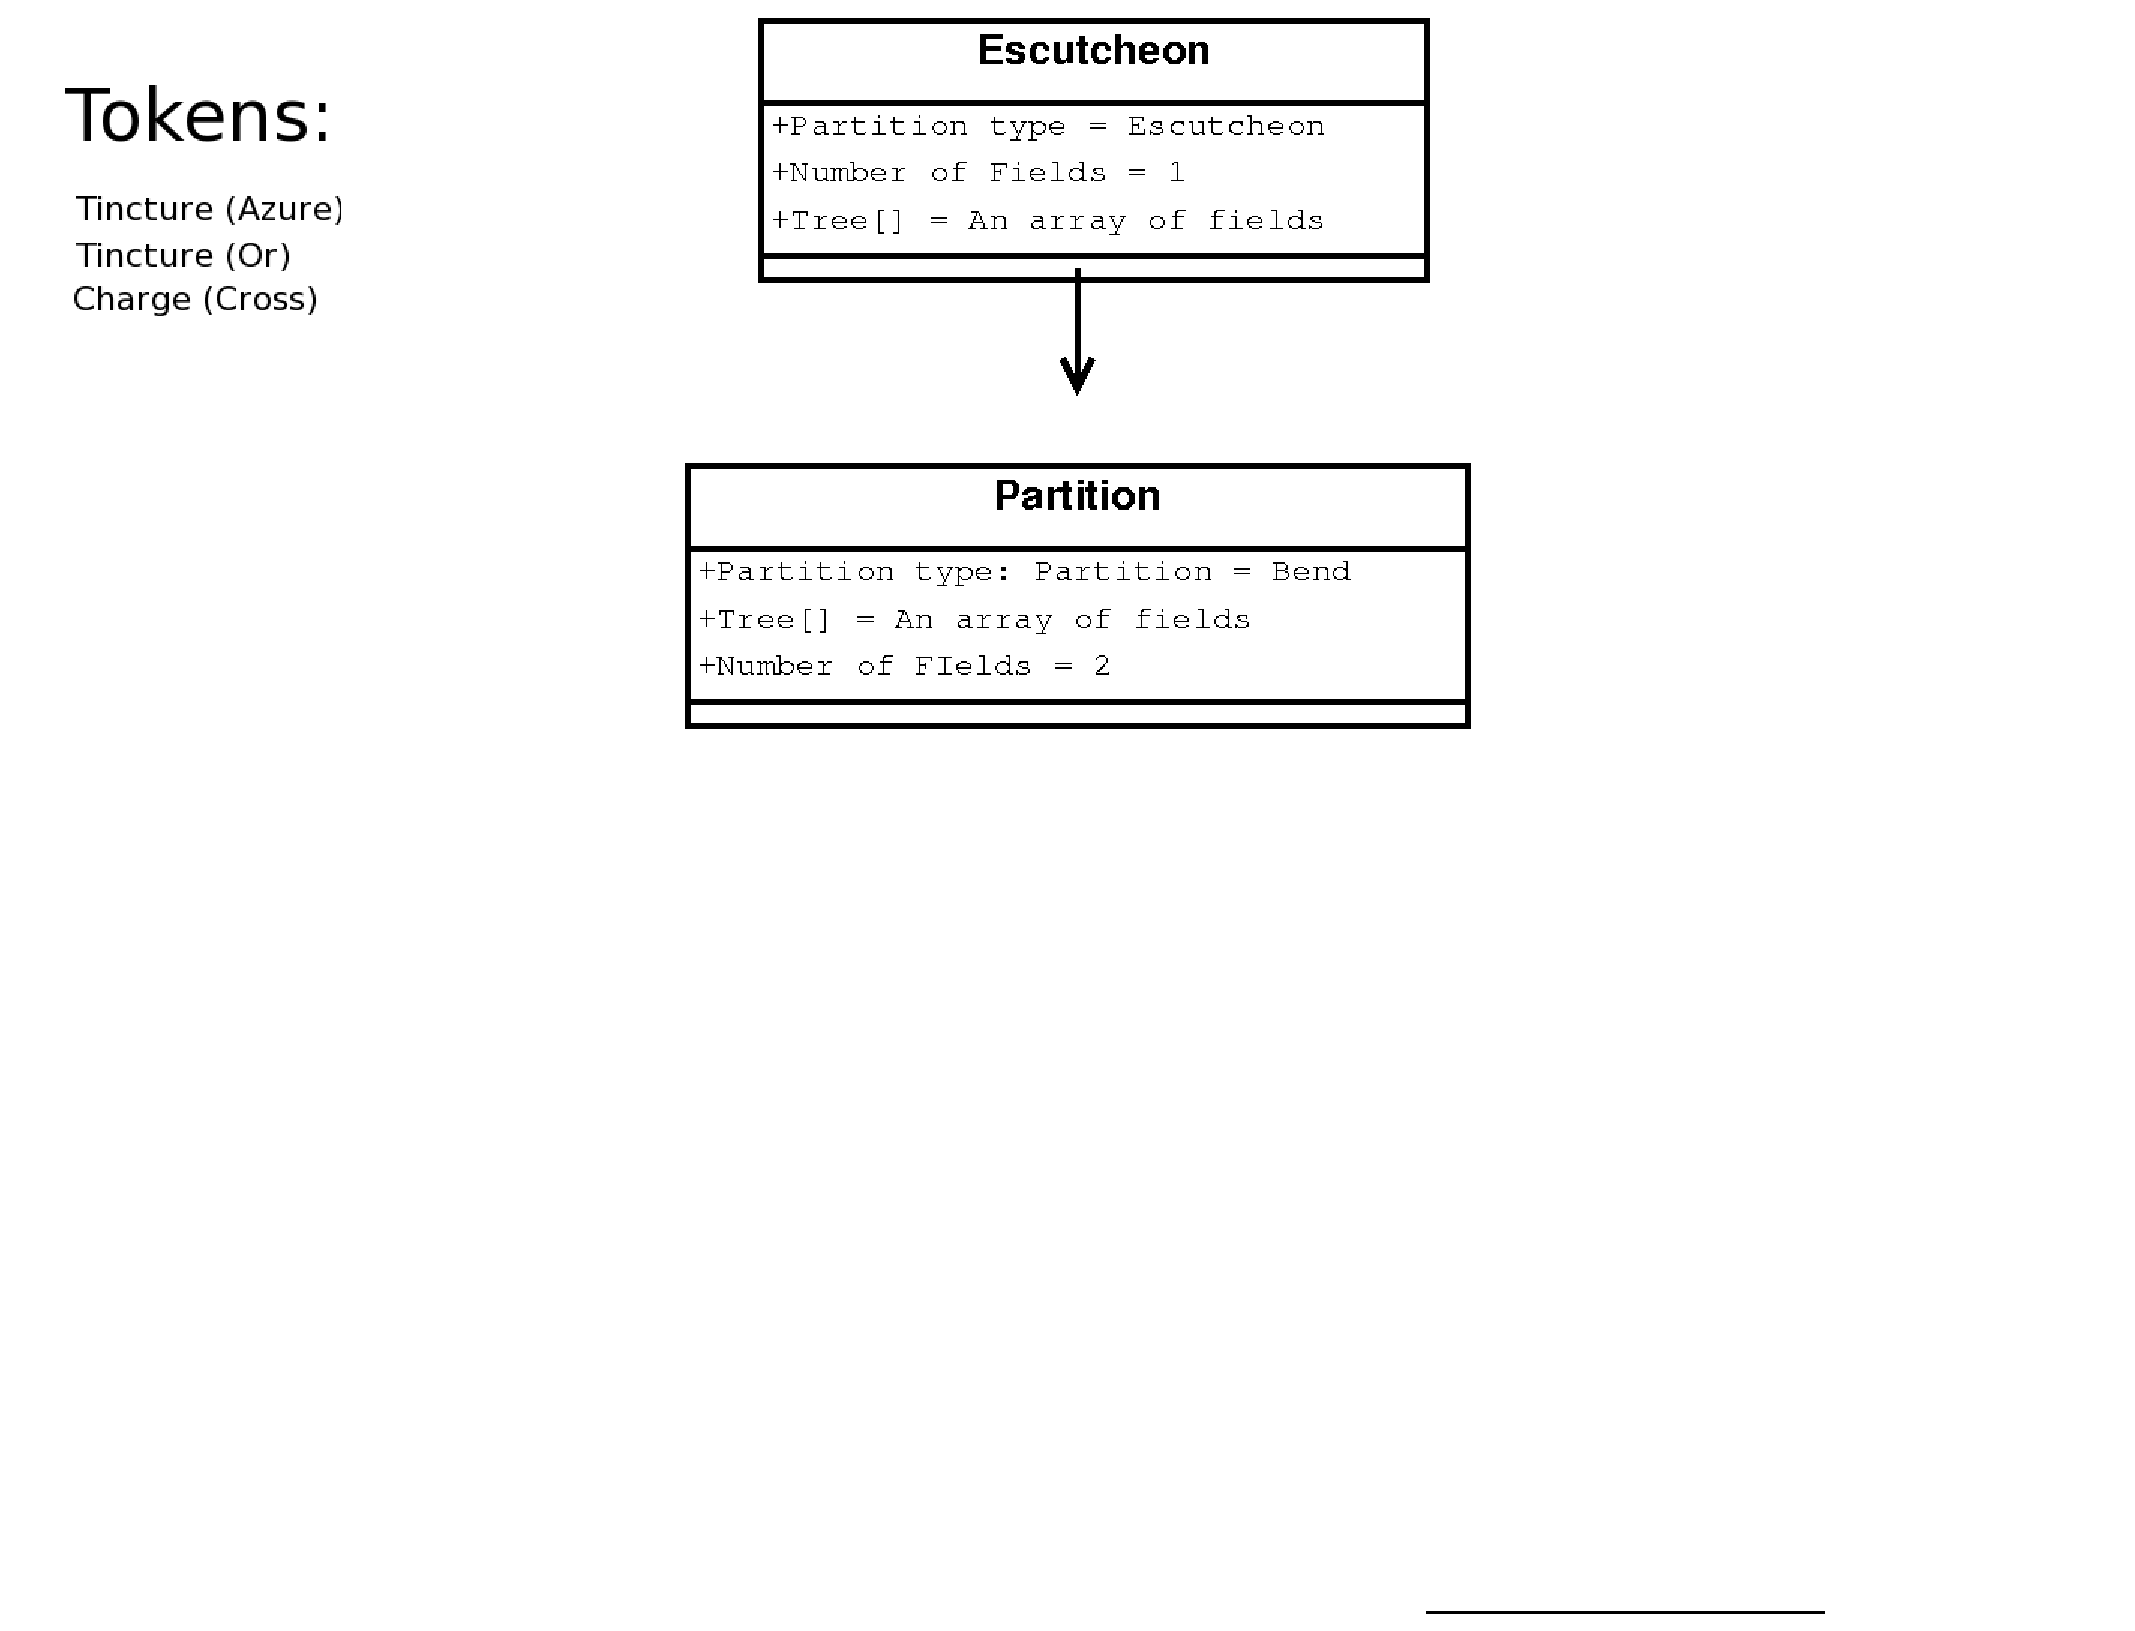
\includegraphics[width=0.8\textwidth]{parsing/images/Parsing4.eps}
  \caption{\emph{"The first token is checked against the grammar then added to the tree array of the initial field."}}
  
\end{figure}


\begin{figure}[H]
  \centering
    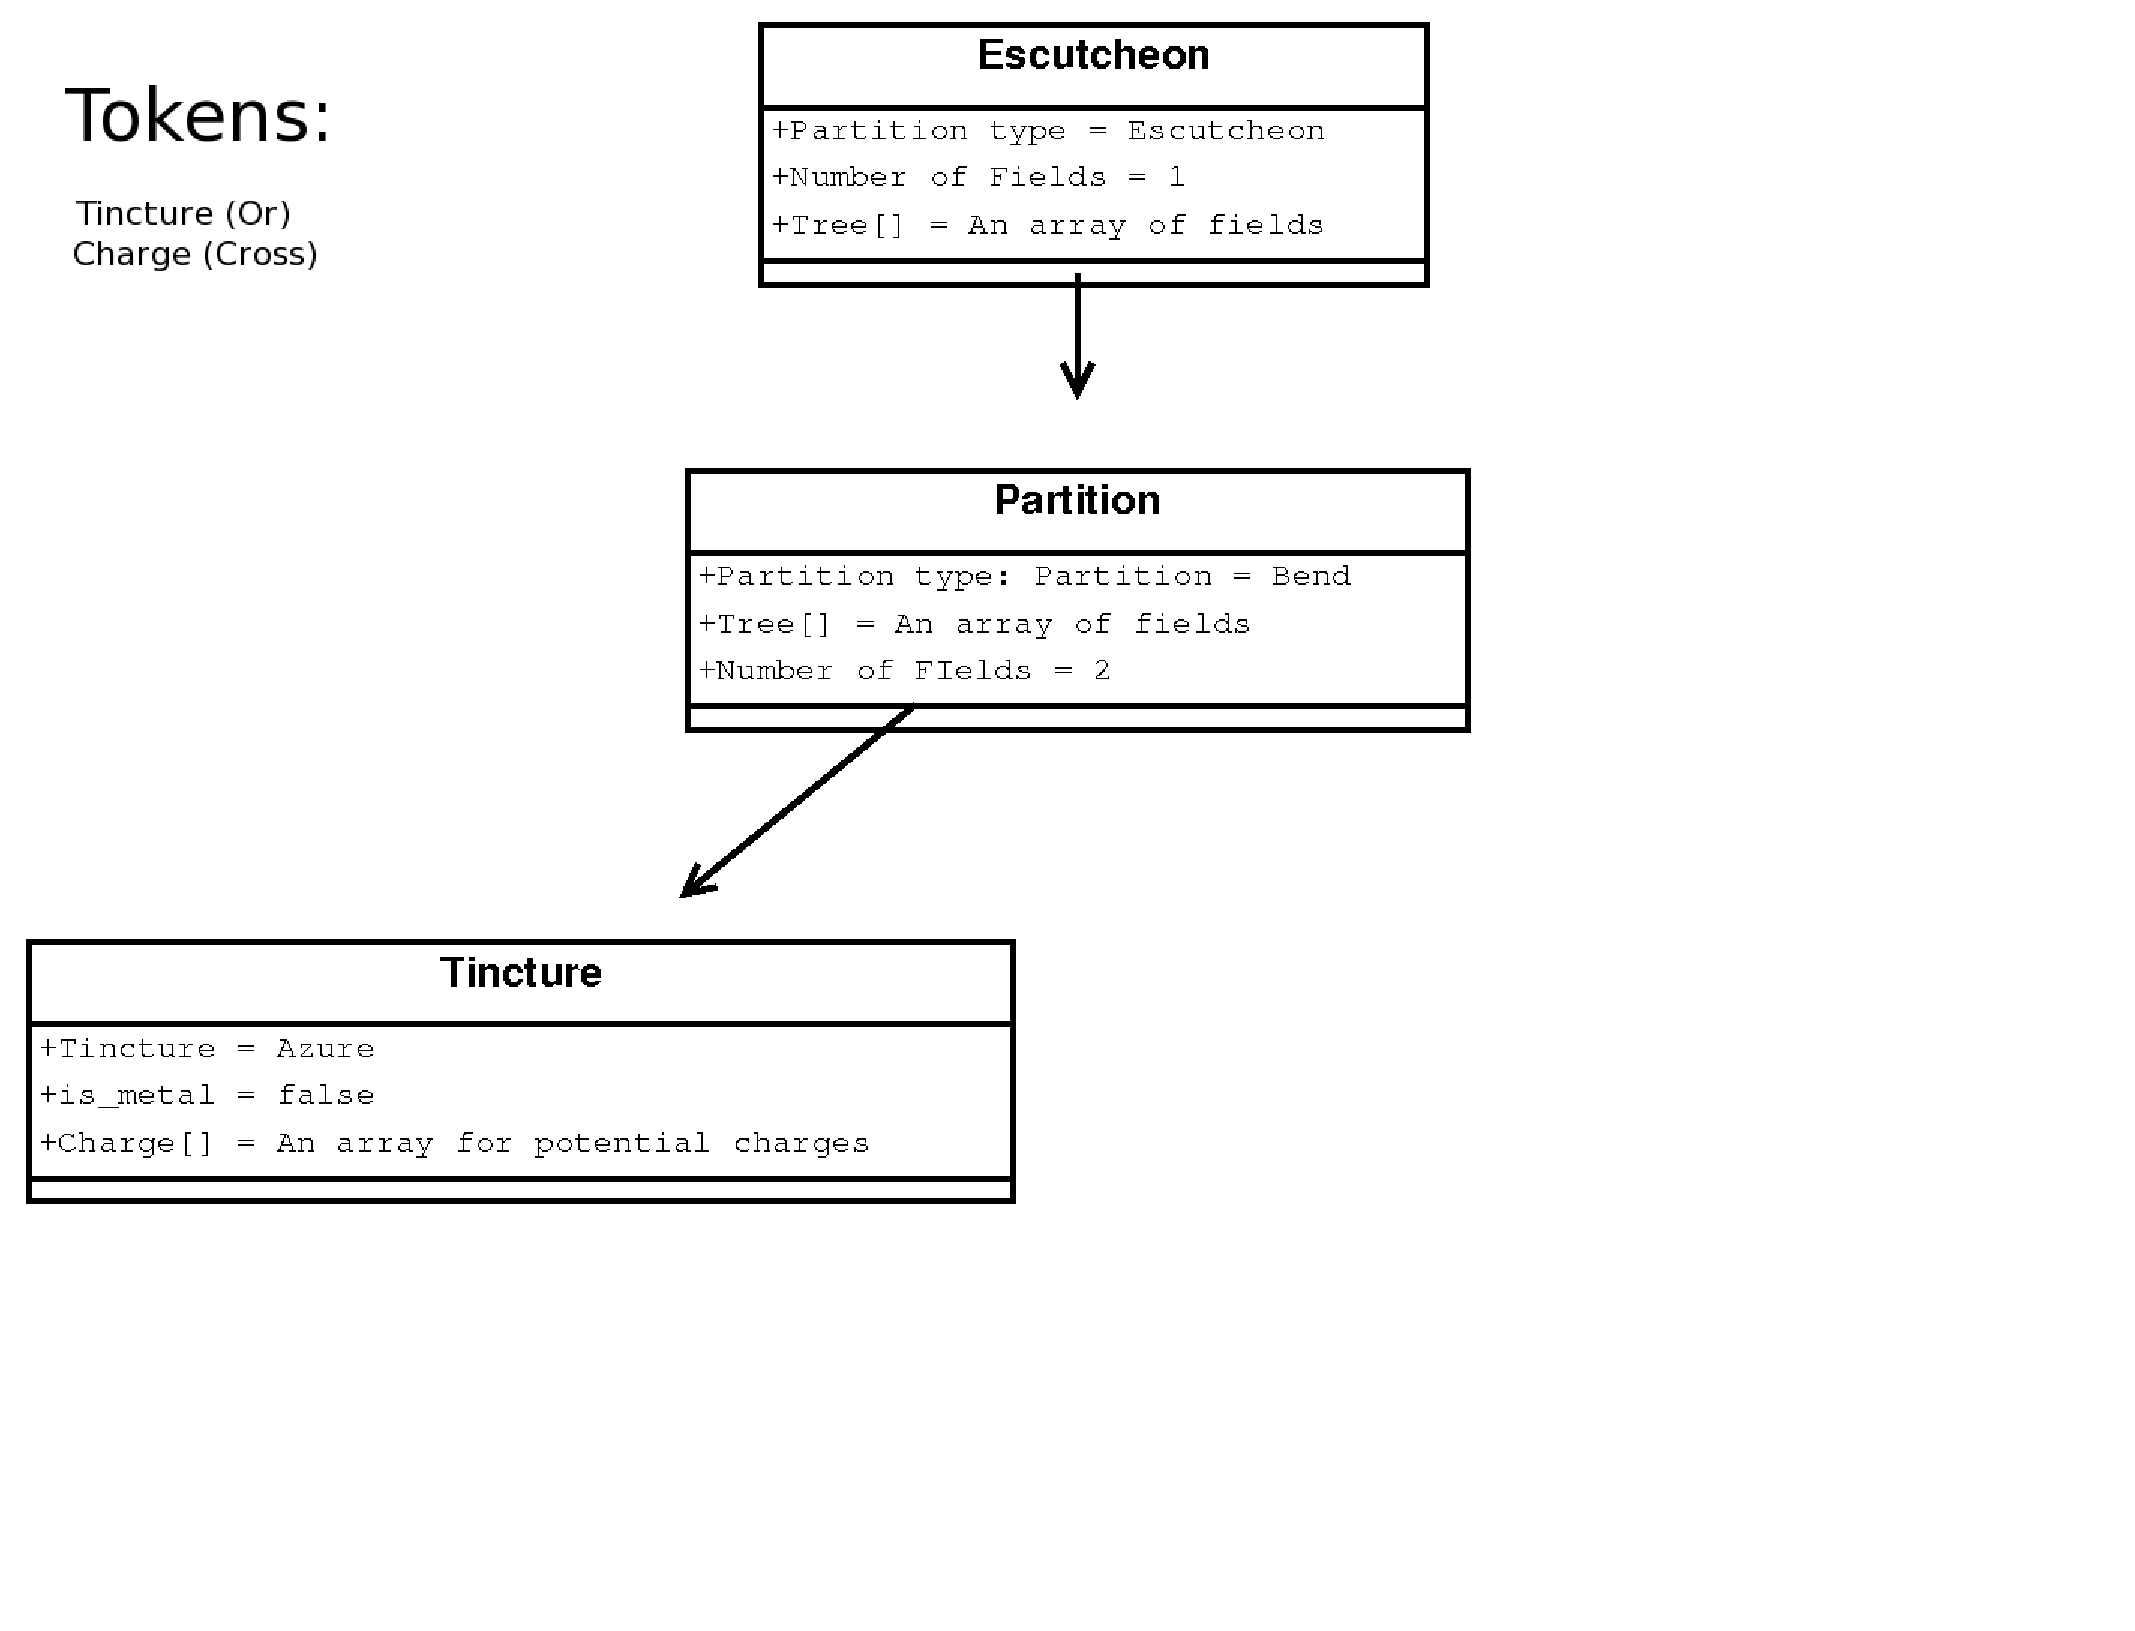
\includegraphics[width=0.8\textwidth]{parsing/images/Parsing3.eps}
  \caption{\emph{"The next token is a Tincture so the first element of the Bend's tree array is assigned to this Tincture"}}
  
\end{figure}

\begin{figure}[H]
  \centering
    \includegraphics[width=0.8\textwidth]{parsing/images/Parsing2.eps}
  \caption{\emph{"The next token is another Tincture so the last element in the Bend's tree array is assigned to this Tincture."}}
  
\end{figure}

\begin{figure}[H]
  \centering
    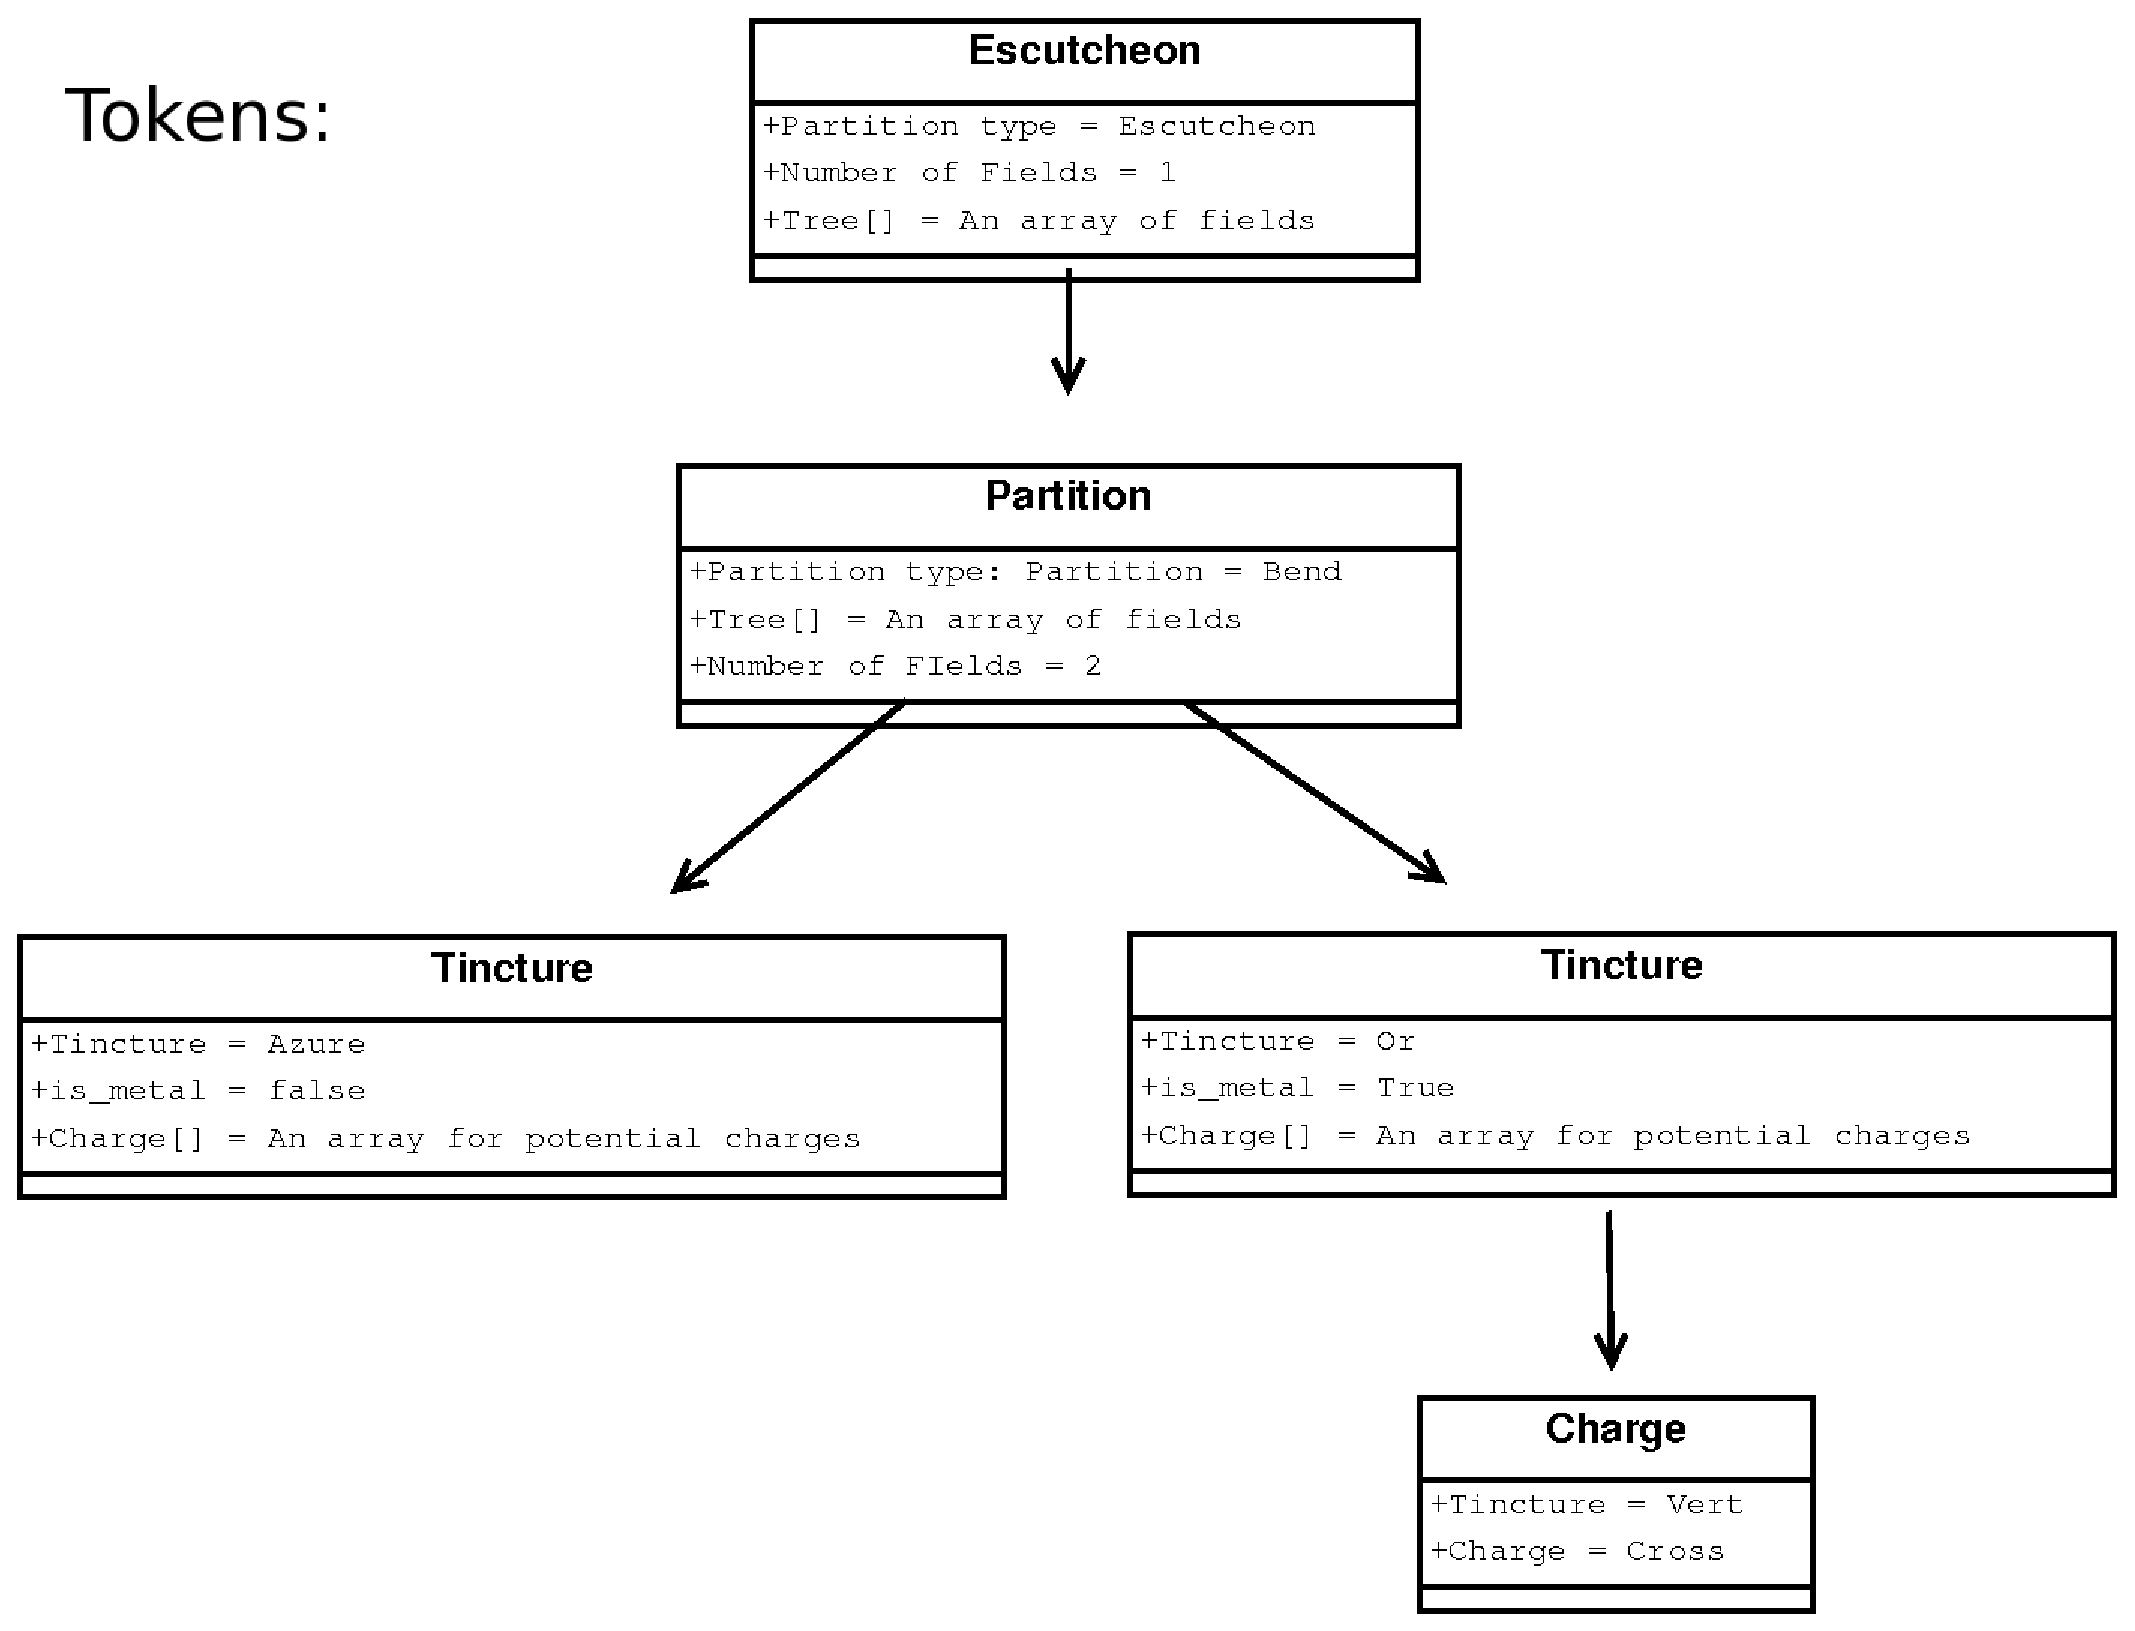
\includegraphics[width=0.8\textwidth]{parsing/images/Parsing1.eps}
  \caption{\emph{"The final token is a Charge as the last token was a Tincture this is a valid token.  The Charge is assigned to the first element of the Or's charge array. As there are no more tokens and no more empty fields this is a valid Blazon sentence and has finished being Parsed."}}
  
\end{figure}



% figures demonstrating parsing




\section{Error handling}

If there are no more tokens but the tree has empty nodes in it then the Blazon sentence is invalid because at least one field has yet to be tinctured.  If the inverse is true and there is no space in the tree for the next Token then too many field have been defined.